\section{Initial Results: Gradient Descent}

In trying to tackle this inverse problem as a quadratic, I've considered that I need to approach the problem from a different angle.
Many of the methods we've discussed in class won't necessarily apply directly to the problem.
Particularly, three different methods seem to work best in combatting quadratic inverse problems:

\begin{itemize}
    \item Linearize the problem
    \item Use optimization techniques
    \item Use specialized algorithms
\end{itemize}

The methods used in~\cite{grindrod2009} seem to fall under a specialized algorithm, as they perform case analysis
on the eigenanalysis of $\delta_R$.
My immediate reaction was to attack the problem as an optimization problem, as I have experience in this
both in this course and in solving other problems.

I began by implementing a gradient descent algorithm to solve the problem.
To test this solution, I directly created 200 states of a graph using a random range-dependency $q$.
For two vertices with range $k$, they have a birth rate $\alpha (k) = 0.1(0.98^{k^2})$ and death rate $\omega (k) = 0.2$.
Then, I ran my algorithm on these states to learn a mapping $q'$, then ran another walk $q'$ to generate
new states of the graph.
Assuming that the birth and death rates of the graph are similar, these simulations should result in very similar graphs
after 200 iterations.
See Figure ~\ref{fig:gradient-accuracy} for the results of this experiment.
Overall, this is a very solid fit. You can see that my algorithm ends up with nearly the same graph.

\begin{figure}
    \begin{minipage}{0.49\textwidth}
        \begin{center}
            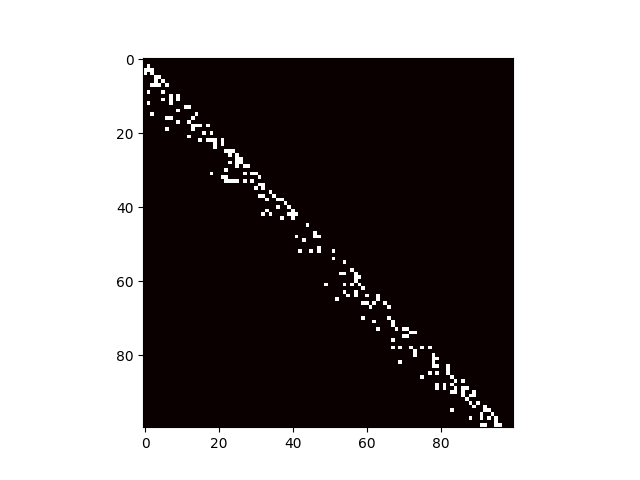
\includegraphics[scale=0.5]{figures/original_adj_100.png}
        \end{center}
    \end{minipage}
    \begin{minipage}{0.49\textwidth}
        \begin{center}
            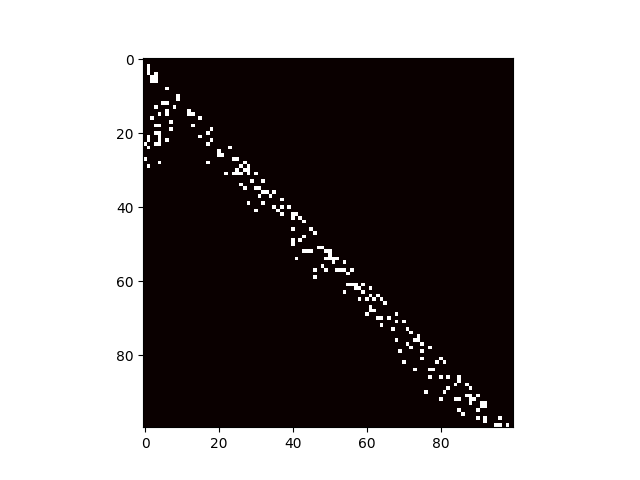
\includegraphics[scale=0.5]{figures/sgd_adj_100.png}
        \end{center}
    \end{minipage}
	\caption{
        Left: State 200 of the original graph. 
        This range-dependent mapping has error = 1.2M.
        Right: State 200 of the graph with a range mapping learned by gradient descent.
        Note that the mapping is mostly accurate, but gets caught in a local minimum
        where the vertices in the top left have been mapped inoptimally.
        This range-dependent mapping has error = 1.6M
	}
    \label{fig:gradient-accuracy}
\end{figure}